\documentclass[11pt]{article}
\usepackage[utf8]{inputenc}
\usepackage[T1]{fontenc}
\usepackage[francais]{babel}
\usepackage[francais]{layout}
\usepackage{hyperref}
\selectlanguage{french}
\usepackage[toc,page]{appendix}


%\usepackage[dvipsnames]{xcolor}


% NE PAS CHANGER !!
\ifx \public \undefined \def\public{etudiants} \fi
%\ifx \public \undefined \def\public{enseignants} \fi
\usepackage[\public]{tps}
\usepackage{tikz}

\usepackage{hyperref}
\hypersetup{
    colorlinks=true,
    linkcolor=blue,
    filecolor=magenta,      
    urlcolor=cyan,
}

\urlstyle{same}



% Numéro du TP
\newcommand{\numtd}{03}
% Titre du TP
\newcommand{\titretd}{Data Representation}
\def\tup#1{\langle #1\rangle}
\begin{document}
	
	\entete{\numtd}{\titretd}


\subsection*{Warming up:}
For the 16-bit codes: $0000 0000 0010 1010$ and $1000 0000 0010 1010$ Give their values, if they are representing:

\begin{itemize}
    \item a 16-bit unsigned integer;
    \item a 16-bit signed integer;
    \item two 8-bit unsigned integers;
    \item two 8-bit signed integers;
    \item a 16-bit Unicode characters;
    \item two 8-bit ISO-8859-1 characters
\end{itemize}

\bigskip

How would you represent "Hello, how are you?" in ASCII? (look for the comma, question mark, and space characters in the ASCII table)

\begin{solution}
\begin{itemize}
	\item 42, 32810
	\item 42, 32726
	\item 0,42; 128,42
	\item 0,42; -128,42
	\item * and 
	%\begin{figure}[h!]
%		\centering
%		\label{fig:802a}
	
\includegraphics[scale=0.1]{802a.png}
%		\caption{UTF-16 802A}
%	\end{figure}
	\item null, * and undefined
	\item 72 101 108 108 111 44 32 104 111 119 32 97 114 101 32 121 111 117 32 63 
\end{itemize}	
\end{solution}



\section{Analyzing an error}


\subsection{In the html pages}
Visit the \url{https://amritasuresh.github.io/encoding.html}\bigskip. Describe what is happening using the tables of characters available on the internet (\url{https://fr.wikipedia.org/wiki/Table_des_caractères_Unicode_(0000-0FFF)}). 
And provide a solution to correct this problem.


\begin{solution}

Nous sommes face à un problème d'encodage. Les caractères spéciaux s'affichent
sur deux ou trois caractères au lieu d'un. Il semble que nous soyons face à une
page UTF-8 interprétée en ISO8859-1.

\begin{itemize}
\item é : à = 00c3 soit 11000011 ; © = 00a8 soit 10101000
\item ç :
\item Ã\"{ } : 
\end{itemize}

\end{solution}



\section{File encoding problem}
Download the text file \url{http://www.lsv.fr/~fhh/tp05-2.txt} and view it in your browser.

Search "é" with Firefox and Chrome.

Search "é" with the command "grep" on the downloaded file. 

What do you see? 

Suggest a solution to correct this type of problem.


\begin{solution}
Les <<é>> sont codés de deux manière différentes. <<hexdump -C>> donne les codages des caractères.

Solution utiliser uconv -x NFD avant de mettre ce type de fichier dans une base de donnée.
\end{solution}


\section{Character encoding in HTML}
HTML pages have several ways to encode characters:
\begin{itemize}
	\item Entity references which is an alternative name for a series of characters. You can use an entity in the \texttt{\&name;} format, where name is the name of the entity
	\item Numeric references that give the code of a Unicode character, in the form 
	\texttt{\&\#}\emph{nnn}\texttt{;} (décimal) or
	\texttt{\&\#x}\emph{nnn}\texttt{;}.\smallskip
	\item Direct binary coding in one of the formats discussed in the course (UTF-8, ISO-8859-1, \ldots). This requires adding a tag of the form
	\begin{quote}
		\texttt{<meta http-equiv="Content-Type" content="text/html; charset=iso-8859-1" />}
	\end{quote}
	in the \texttt{header} of the HTML document.
\end{itemize}
We will consider the names of the following European municipalities:
\begin{quote}
	Crèvec\oe{}ur (France)\\ L'Ha\"y-les-Roses (France)\\ Krom\v{e}\v{r}\'i\v{z}
	(Tchéquie)\\ G\"od\"oll\H{o} (Hongrie)\\ S\"u\ss{}en (Allemagne)\\
	Pr\ae{}st\o{} (Danemark)
\end{quote}

\begin{enumerate}
	\item Create an HTML document that displays these names with their entity references.
	\item Look for Unicode codes for non-ASCII characters and use them to recreate the list with numeric references.
	\item Create an HTML document in UTF-8 directly with your text editor.
\end{enumerate}




\section{Huffman Encoding}
As we have seen in ASCII, every character is encoded with the same number of bits: 8 bits per character. Since there are 256 different values that can be encoded with 8 bits, there are potentially 256 different characters in the ASCII character set -- note that $2^8 = 256$. The common characters, e.g., alphanumeric characters, punctuation, control characters, etc., use only 7 bits; there are 128 different characters that can be encoded with 7 bits. In C++ for example, the type char is divided into subtypes unsigned-char and (the default signed) char. As we'll see in this exercise, Huffman coding compresses data by using fewer bits to encode more frequently occurring characters so that not all characters are encoded with 8 bits.

Huffman coding provides an efficient, unambiguous code by analyzing the frequencies that certain symbols appear in a message. Symbols that appear more often will be encoded as a shorter-bit string while symbols that aren't used as much will be encoded as longer strings. Since the frequencies of symbols vary across messages, there is no one Huffman coding that will work for all messages. This means that the Huffman coding for sending message X may differ from the Huffman coding used to send message Y. There is an algorithm for generating the Huffman coding for a given message based on the frequencies of symbols in that particular message.

Huffman coding works by using a frequency-sorted binary tree to encode symbols.

We'll look at how the string "go go gophers" is encoded in ASCII, how we might save bits using a simpler coding scheme, and how Huffman coding is used to compress the data resulting in still more savings.

\begin{enumerate}
	\item With an ASCII encoding (8 bits per character) as seen below the 13 character string "go go gophers" requires 104 bits. 
	\begin{verbatim}
		char		ASCII		binary
		g				   103			  1100111
		o				   111			  1101111
		p				  112			  1110000
		h				   104			  1101000
		e				   101			   1100101
		r				   114			  1110010
		s				   115			  1110011
		space		32		  1000000
		
	\end{verbatim}
Do you have a suggestion on how to reduce this size if the ONLY phrase we needed to represent was "go go gophers"? How many bits would you need?
\end{enumerate}

By using the above strategy, the string "go go gophers" uses a total of 39 bits instead of 104 bits. More bits can be saved if we use fewer bits to encode characters like g, o, and space that occur frequently and more bits to encode characters like e, p, h, r, and s that occur less frequently in "go go gophers". This is the basic idea behind Huffman coding: to use fewer bits for more frequently occurring characters. 

Encodings can either be fixed-length or variable-length.

\begin{figure}[h!]
	\centering
	\label{fig:encoding-1}
	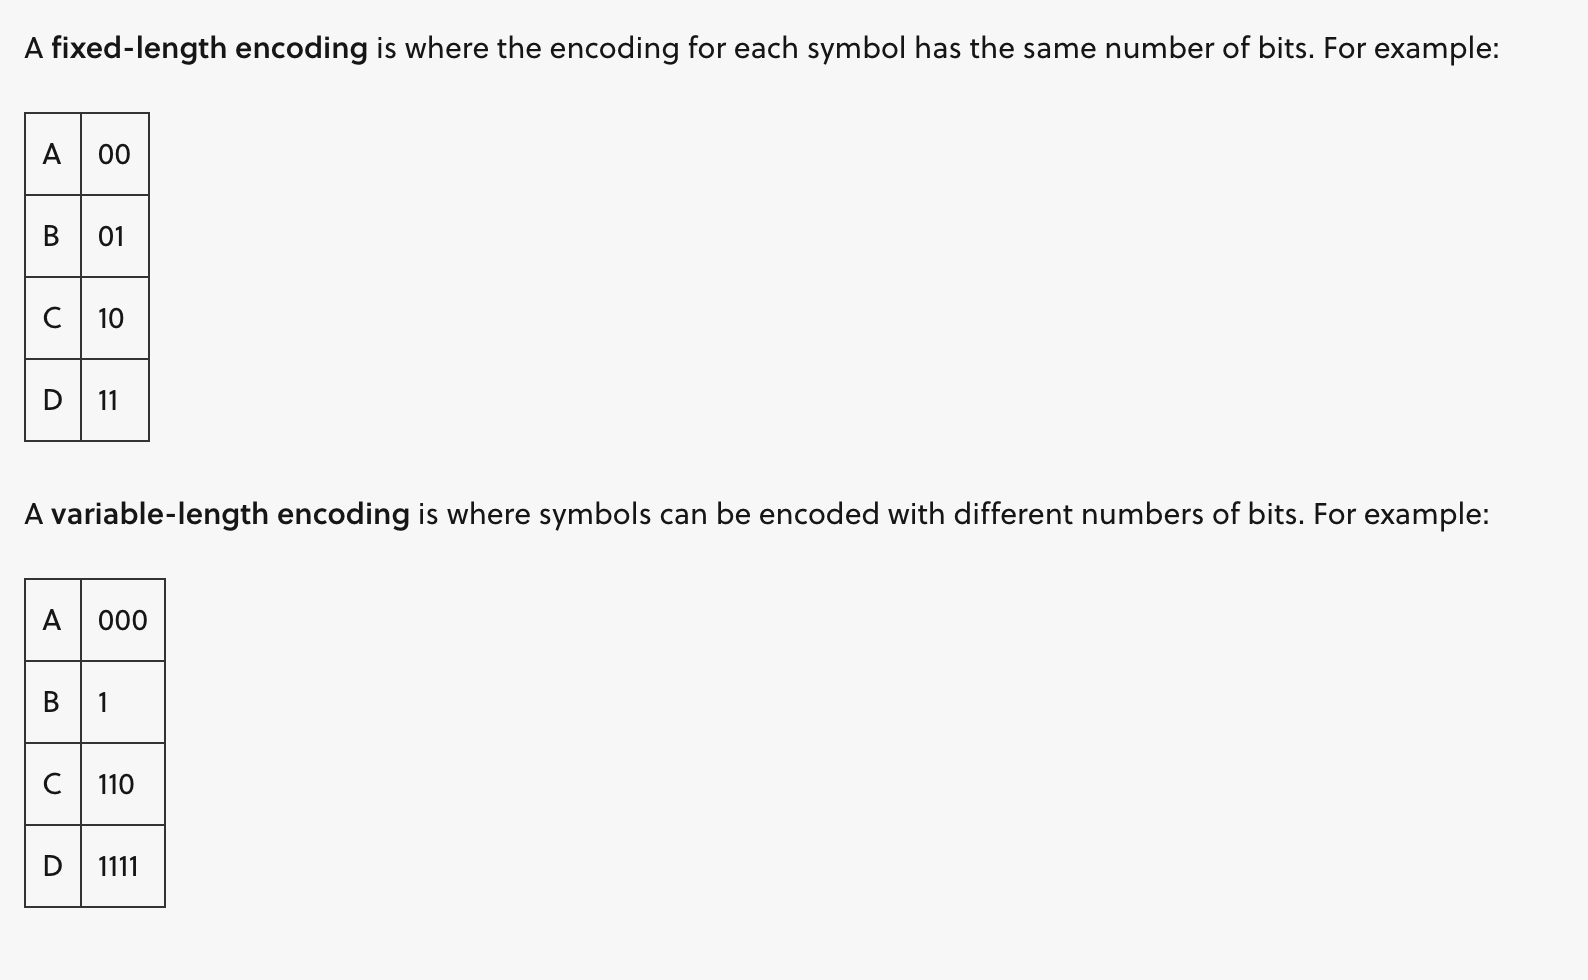
\includegraphics[scale=0.5]{encoding-1.png}
	\caption{Encoding schemes}
\end{figure}

\begin{enumerate}\setcounter{enumi}{1}
	\item Explain why the encoding scheme below is a poor encoding (we shall call this Encoding-A) (we assume that our text has the words A and B more frequently, and C and D less frequently).
	\begin{verbatim}
		A		0
		B		1
		C		11
		D		10
	\end{verbatim}
What value is encoded as "01110" in the above encoding?

\item The encoding below is unambiguous, but inefficient since there exists a shorter (and still unambiguous) encoding of these letters. Give an equivalent but shorter encoding.

	\begin{verbatim}
	A		0000			
	B		0101
	C		1010
	D		1111
\end{verbatim}
How many bits are needed to represent $n$ different symbols (using fixed-length encoding)?

\item With Encoding-A as the encoding, construct a binary tree such that "some" of the nodes of the tree correspond to the symbols (in this case A, B, C, D), and the assignment will be the path it takes to get from the root of the tree to that leaf.
What do you notice about the tree?

\end{enumerate}

As shown above, it is important for an encoding scheme to be unambiguous. Since variable-length encodings are susceptible to ambiguity, care must be taken to generate a scheme where ambiguity is avoided. Huffman coding uses a greedy algorithm to build a prefix tree that optimizes the encoding scheme so that the most frequently used symbols have the shortest encoding. The prefix tree describing the encoding ensures that the code for any particular symbol is never a prefix of the bit string representing any other symbol. To determine the binary assignment for a symbol, make the leaves of the tree correspond to the symbols, and the assignment will be the path it takes to get from the root of the tree to that leaf.

\begin{enumerate}\setcounter{enumi}{4}
	\item What encoding do we get from the following Huffman tree?
	\begin{figure}[h!]
		\centering
		\label{fig:encoding-2}
		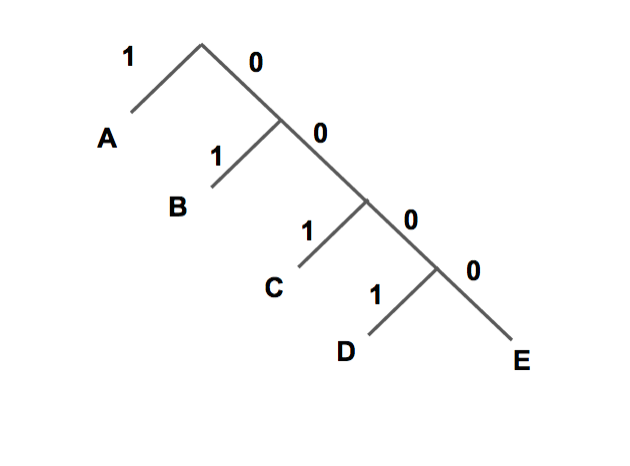
\includegraphics[scale=0.5]{encoding-2.png}
	\end{figure}
\end{enumerate}

The Huffman coding algorithm takes in information about the frequencies or probabilities of a particular symbol occurring. It begins to build the prefix tree from the bottom up, starting with the two least probable symbols in the list. It takes those symbols and forms a subtree containing them, and then removes the individual symbols from the list. The algorithm sums the probabilities of elements in a subtree and adds the subtree and its probability to the list. Next, the algorithm searches the list and selects the two symbols or subtrees with the smallest probabilities. It uses those to make a new subtree, removes the original subtrees/symbols from the list, and then adds the new subtree and its combined probability to the list. This repeats until there is one tree and all elements have been added.

\begin{enumerate}\setcounter{enumi}{5}
	\item Given the following probability table, create a Huffman tree to encode each symbol.
	\begin{verbatim}
	Symbol		Probability
	A		   		   0.3
	B		   		   0.3
	C		   		   0.2
	D		   		   0.1
	E		   		   0.1
	\end{verbatim}
\item How many bits do you need to create a Huffman coding for this probability table?
	\begin{verbatim}
	Symbol		Probability
	A		   		   0.6
	B		   		   0.1
	C		   		   0.1
	D		   		   0.1
	E		   		   0.1
\end{verbatim}

%\item What is complexity of constructing a Huffman coding, if we know the characters and their probabilities in advance?

\item When do you think this encoding is optimal? When is it not?
\end{enumerate}

\end{document}
